\section {Task Formulation}

\begin{figure}[t]
\centering
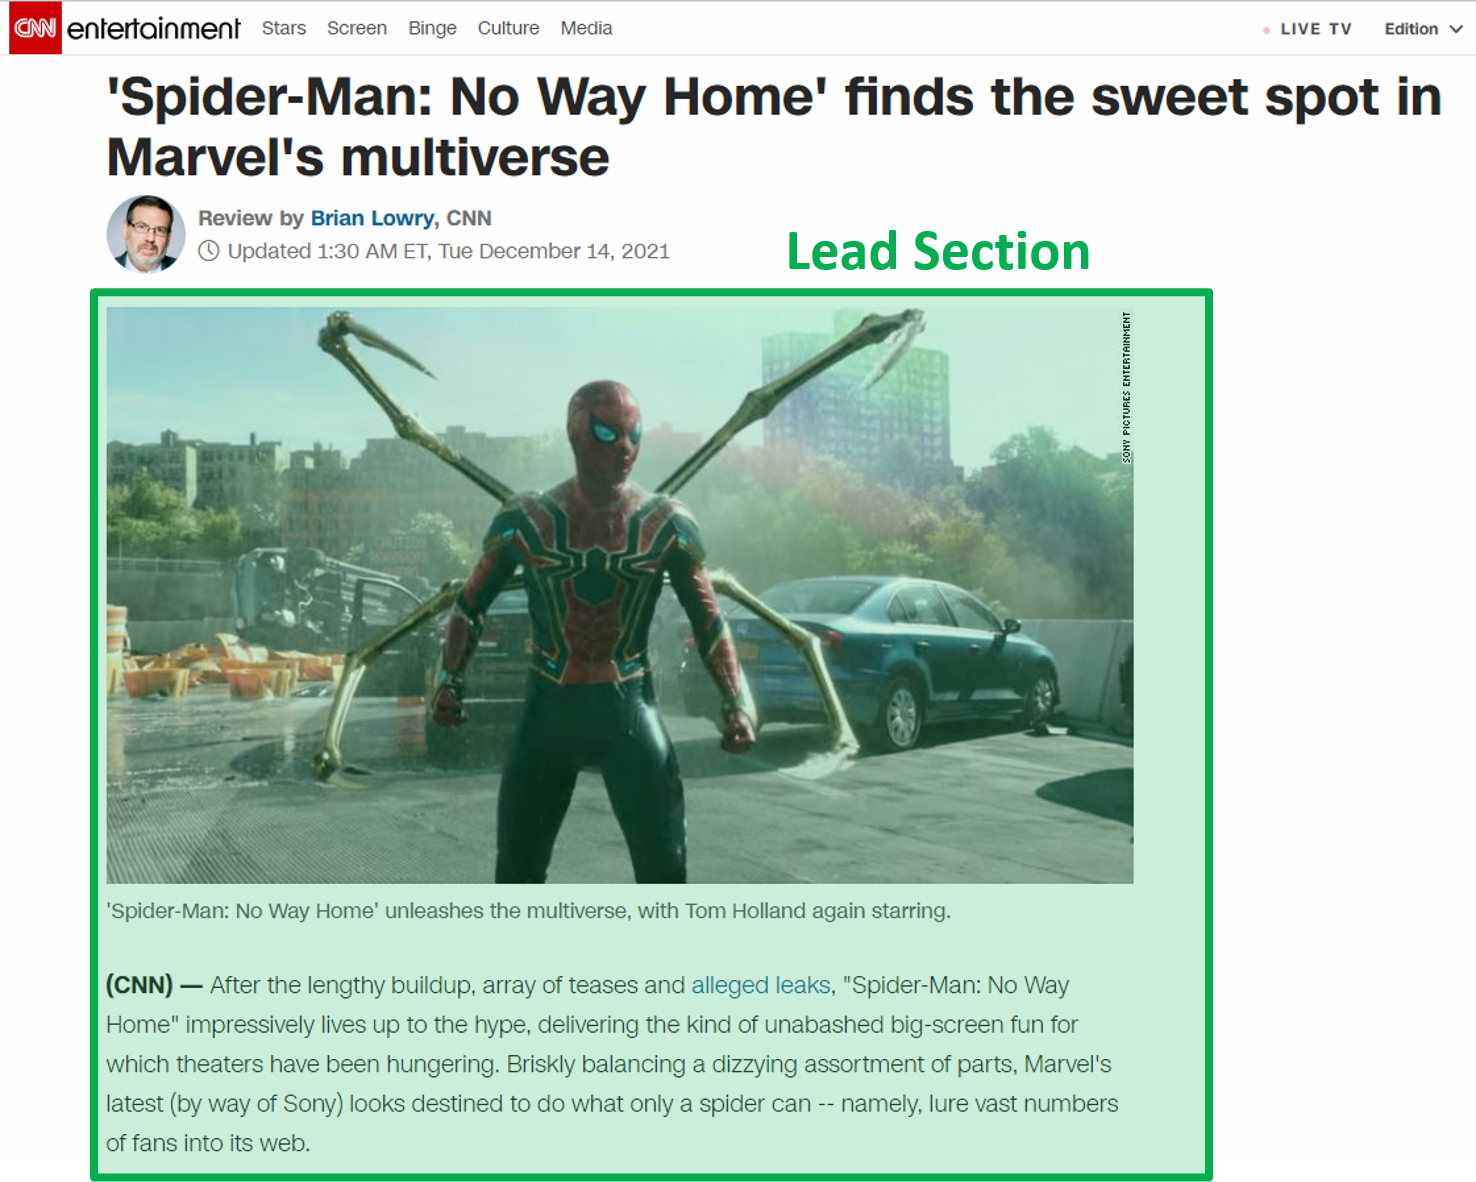
\includegraphics[width=1\columnwidth]{vis_example1}
\caption{The structure of a sample article with the lead section (green shading)}
\label{vis_example1}
\end{figure}

The set of articles is $P = \{p_1, p_2, \cdots, p_n\}$. For each article $p_i$, it gets viewed by $v_i$ times in a certain period of time. Given a page $p$ which has been viewed for $v$ times, for any hyperlink $l$ on this page, we define the click counts of this hyperlink as $click(p, l)$ and the click through rate can thus be represented as $ctr(p,l) = click(p,l) / v$. The click through rate $ctr(p, l)$ is then used as our ground truth.

In this paper, our task is to rank the hyperlinks according to their click through rate $ctr(p,l)$. We consider two tasks: source link ranking and target link ranking. Given a certain page $p$, source links are those hyperlinks directing to page $p$ and target link are those hyperlinks appeared on page $p$ and directs to target article. The corresponding set of links $L$ for page $p$ are thus different in these two situations. We use $L^s_i$, $L^t_i$ to represent the corresponding set of source/target links for article $p_i$, where $L^s_i = \{l^s_1, l^s_2, \cdots, l^s_{N^s_i}\}$ and $N^s_i = |L^s_i|$, and similar notations goes for $L^t_i$ and $N^t_i$. 

For the ranking of target links, given an article $p_i$, every target link $l^t_j \in L^t_i$ has its corresponding label $y_j$ indicating its true ranking. Ranking hypertext links can be viewed as a task of finding permutation $\pi = \{y
^*_1, y^*_2, \cdots, y^*_{N^t_i}\}$ on indices $\{1,2,\cdots,N^t_i\}$. Each hyperlink $l^t_j$ on the pages can be characterized by a feature vector $\vec{x_j}$. The Learning to Rank algorithm then automatically learns a model to predict the true ranking of link $l^t_j$ from all the feature vectors. The ranking of source links is similar, but within $L^s_i$.